%%%%%%%%%%%%%%%%%%%%%%%%%%%%%%%%%%%%%%%%%%%%%%%%%%%%%%%%%%%%%%%%%%%%%%%%%
%%   APPENDIX: MISCELLANEOUS MATH
%%%%%%%%%%%%%%%%%%%%%%%%%%%%%%%%%%%%%%%%%%%%%%%%%%%%%%%%%%%%%%%%%%%%%%%%%

\renewcommand{\chapterfolder}{appendices/}
\chapterimage{cover/appendix_math}

\chapter{Mathematical Miscellany}\label{app:math}

In this appendix, we present some of the miscellaneous bits of mathematical knowledge that we needed to discuss certain concepts or to prove certain theorems. While none of these topics are particularly deep, they are often taught at scattered places throughout one's math education (or not taught at all), so we summarize them here for ease of reference.


%%%%%%%%%%%%%%%%%%%%%%%%%%%%%%%%%%%%%%%%%%%%%%%%%%%%%%%%%%%%%%%%%%%%%%%%%
%%   SECTION: MODULAR ARITHMETIC
%%%%%%%%%%%%%%%%%%%%%%%%%%%%%%%%%%%%%%%%%%%%%%%%%%%%%%%%%%%%%%%%%%%%%%%%%
\section{Modular Arithmetic}\label{sec:modular_arithmetic}

To be filled in later. Maybe not actually needed?


%%%%%%%%%%%%%%%%%%%%%%%%%%%%%%%%%%%%%%%%%%%%%%%%%%%%%%%%%%%%%%%%%%%%%%%%%
%%   SECTION: GREATEST COMMON DIVISOR
%%%%%%%%%%%%%%%%%%%%%%%%%%%%%%%%%%%%%%%%%%%%%%%%%%%%%%%%%%%%%%%%%%%%%%%%%
\section{Greatest Common Divisor and Least Common Multiple}\label{sec:gcd}

The \emph{greatest common divisor} (or \emph{GCD} for short) of two non-zero integers $a$ and $b$ is the largest positive integer that evenly divides both $a$ and $b$. We often denote the GCD of $a$ and $b$ by $\mathrm{gcd}(a,b)$. For example, $\mathrm{gcd}(6,15) = 3$. Our primary interest in the GCD comes from the fact that it tells us exactly which equations of the form $ax + by = c$ (where $a,b,c$ are given integers, and $x,y$ are variables we are trying to solve for) have integer solutions.\footnote{An equation of this form is called a \emph{linear Diophantine equation}.} In particular, the following theorem answers this question:

% TODO: Add example to illustrate this theorem, as well as GCD/LCM stuff. This is really opaque for this level of book right now.

\begin{theorem}[B\'ezout's identity]\label{thm:linear_diophantine}
	Let $a, b,$ and $c$ be non-zero integers. Then the equation $ax + by = c$ has a solution where both $x$ and $y$ are integers if and only if $c$ is a multiple of $\mathrm{gcd}(a,b)$. Furthermore, if $a$ and $b$ have opposite signs then $x$ and $y$ can be chosen to both be positive.
\end{theorem}

\begin{proof}
	To prove the ``only if'' direction of the theorem, we note that $\mathrm{gcd}(a,b)$ evenly divides each of $a$ and $b$, so for all integers $x,y$ it evenly divides $ax + by$ as well, so $c$ must be a multiple of $\mathrm{gcd}(a,b)$.
	
	To prove the ``if'' direction of the theorem, we suppose that $c$ is a multiple of $\mathrm{gcd}(a,b)$, and we will show that there exist integers $x,y$ such that $ax+by = c$. To this end, let $x^\prime$ and $y^\prime$ be integers that make $ax^\prime + by^\prime$ as small (but positive) as possible. For convenience, define $s := ax^\prime + by^\prime$. When dividing $a$ by $s$, the remainder $r$ is also of the form $r = ax + by$ since it is obtained by subtracting a multiple of $s = ax^\prime + by^\prime$ from $a$. Since the $0 \leq r < s$, and $s$ is the smallest positive number of this form, the only possibility is that $r = 0$. In other words, $s$ evenly divides $a$ (and a similar argument shows that $s$ evenly divides $b$).
	
	It follows that $c/s$ is an integer (since $c$ is a multiple of $\mathrm{gcd}(a,b)$, which is a multiple of $s$), so $x = x^\prime(c/s)$, $y = y^\prime(c/s)$ is a pair of integers satisfying $ax + by = (ax^\prime + by^\prime)(c/s) = s(c/s) = c$, as desired.
	
	To prove the final claim that $x$ and $y$ can be chosen to be positive when $a$ and $b$ have opposite signs, note that if $x$ and $y$ are integers such that $ax + by = c$ then for any integer $k$ it is also the case that $a(x + k(b/\mathrm{gcd}(a,b))) + b(y - k(a/\mathrm{gcd}(a,b))) = c$. By taking $k$ large enough and positive (if $a < 0$ and $b > 0$) or large enough and negative (if $a > 0$ and $b < 0$), this gives us a positive solution to the equation.
\end{proof}

The \emph{least common multiple} (or \emph{LCM} for short) of two positive integers $a$ and $b$ is the smallest integer that is a multiple of both $a$ and $b$. We often denote the LCM of $a$ and $b$ by $\mathrm{lcm}(a,b)$. For example, $\mathrm{lcm}(6,15) = 30$. It is straightforward to verify that $\mathrm{lcm}(a,b) = ab/\mathrm{gcd}(a,b)$ for all $a,b$.

% Explicitly mention that if gcd(a,n) = 1 then the multiples of a (mod n) reach everything. This idea is used in the silverfish and caterpillar rephasers in chapter 10
% Important: introduce term "relatively prime" and put in the index. This term is used in at least one exercise


%%%%%%%%%%%%%%%%%%%%%%%%%%%%%%%%%%%%%%%%%%%%%%%%%%%%%%%%%%%%%%%%%%%%%%%%%
%%   SECTION: BIG-Theta NOTATION
%%%%%%%%%%%%%%%%%%%%%%%%%%%%%%%%%%%%%%%%%%%%%%%%%%%%%%%%%%%%%%%%%%%%%%%%%
\section{Big-$\Theta$ Notation}\label{sec:bigO}

When describing the long-term behaviour of a Life pattern, we often just want to focus on the ``big picture'', while suppressing the ``fine details''. For example, the pattern displayed in Figure~\ref{fig:max} grows extremely quickly, filling the entire Life plane with zebra stripes\index{aebra stripes} as its four corners expand outward. Patterns that fill the plane like this are called \emph{spacefillers},\index{spacefiller} and this one is called \emph{max}.\footnote{Its name is a reference to the fact that its growth rate is maximal---no pattern can expand faster than $c/2$ in each direction (see Theorem~\ref{thm:speed_limits}), and no pattern can tile the plane with a stable configuration that is more dense than zebra stripes (see Theorem~\ref{thm:still_life_density}).}\index{max}

\begin{figure}[!htb]
	\centering
	\embedlink{max}{\vcenteredhbox{\patternimg{0.093}{max_0}} \vcenteredhbox{\genarrow{100}} \vcenteredhbox{\patternimg{0.093}{max_100}}}
	\caption{The \emph{max} spacefiller. Constructed by Tim Coe in October 1995.}\label{fig:max}
\end{figure}

To communicate how quickly this pattern grows, we could of course give an explicit formula for its population $p(t)$ in generation~$t$, which has the following form:
\begin{align}\label{eq:max_population_formula}
	p(t) = \frac{t^2}{4} + \begin{cases}
		21t/2 + 209, & \text{ if } t \equiv 0 \pmod{4} \\
		21t/2 + 215, & \text{ if } t \equiv 2 \pmod{4} \\
		10t + 923/4, & \text{ otherwise}.
	\end{cases}
\end{align}
However, this formula is quite technical and has many details that we typically do not actually care about. Its ``most important'' piece is the $t^2/4$ term at the front---in the long run (i.e., when $t$ is large), that term has the biggest effect on the population. For this reason, we would typically just say that $p(t)$ ``grows like $t^2/4$'', or even that $p(t)$ ``is proportional to $t^2$''. Big-$\Theta$ notation provides a way of making this terminology precise:

\begin{definition}[Big-$\Theta$ Notation]\label{defn:big_theta}
	Suppose $f$ and $g$ are real-valued functions. We say ``$f(x)$ is $\Theta(g(x))$'' if there exist positive scalars $c$, $C$, and $N$ such that
	\[
		cg(x) \leq f(x) \leq Cg(x) \quad \text{whenever} \quad x \geq N.
	\]
\end{definition}

Informally, the phrase ``$f(x)$ is $\Theta(g(x))$'' means that $f$ and $g$ have the same rate of growth as $x$ gets large, ignoring things like scalars and low-order terms. For example, for the population formula $p(t)$ given in Equation~\eqref{eq:max_population_formula}, we can say that $p(t)$ is $\Theta(t^2)$. This is hopefully somewhat intuitive, but it can be made precise by choosing $c = 1/4$, $C = 1/2$, and $N = 57$ in Definition~\ref{defn:big_theta}---see Figure~\ref{fig:max_population_graph}.\footnote{Many other choices of $c$, $C$, and $N$ are possible as well. For example, we could choose any smaller value of $c$ and/or any larger value of $C$ or $N$. We could even choose a smaller value of $C$ as long as we choose a larger value of $N$ to compensate.}

\begin{figure}[!htbp]
	\centering
	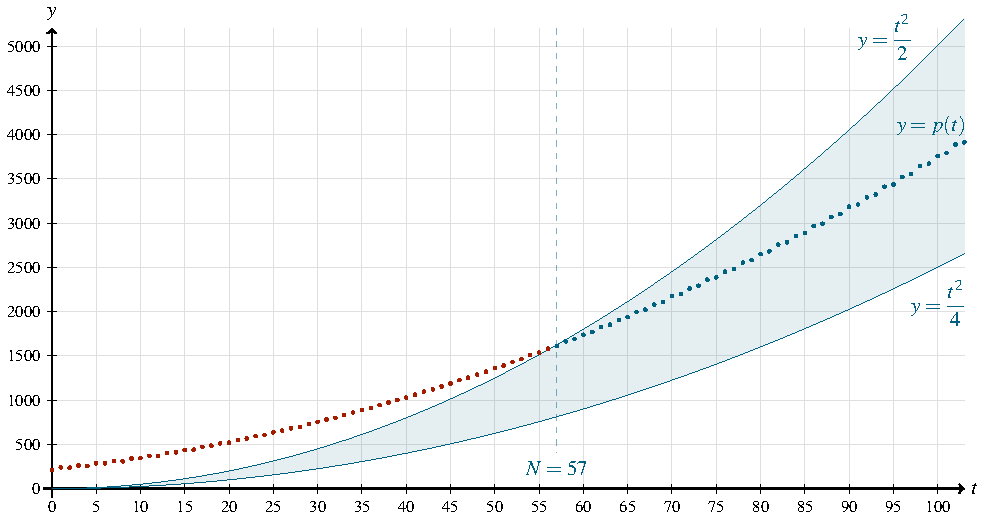
\includegraphics[width=\textwidth]{appendices/max_population.pdf}
	\caption{A plot of the population $p(t)$ of the max pattern from Figure~\ref{fig:max} in generation $t$. Since $p(t)$ is between $t^2/4$ and $t^2/2$ when $t \geq 57$, we say that $p(t)$ is $\Theta(t^2)$.}\label{fig:max_population_graph}
\end{figure}

% TODO: Give a couple more basic mathematical examples? Not motivated by Life, but just things like (any quadratic is Theta(x^2)) and stuff like that?